\subsection{Potential Temperature and Zonal Wind Anomaly}
The zonal-mean potential temperature and potential temperature anomalies for Control, SAI 2020 and SAI 2080 are shown in Figure \ref{fig:th_U_zmdiff_full}, for the annual, JJA and DJF mean. The black countours indicate the zonal-mean zonal wind in m/s. 

In Control we see the potential temperature anomaly signature of increased greenhouse gases, warming at the surface and the troposphere, extending to the lower stratosphere and cooling in the upper stratosphere. The cooling trend in the upper stratosphere is present in SAI 2020 and SAI 2080 as well, but over the Antarctic SAI 2020 and SAI 2080 cool significantly more. With SAI the potential temperature increases where SAI is deployed in the lower stratosphere, conecentrated between 15°S and 30°S around 50 hPa. The warming extends over the Antarctic only in the summer (DJF), because of the lack of incoming solar radiation during the polar night in winter (JJA). The stratosphere in SAI 2020 is about 2.5K warmer than in SAI 2080. The tropospheric temperatures are successfully held at present day values in either SAI scenario, within a margin of $\pm$2.5K.

In JJA (winter) we see that the temperature anomaly in SAI 2020 and SAI 2080 is opposite of the trend in Control. The Antarctic stratosphere cools with SAI instead of warming as it does under global warming. In DJF (summer) the anomaly is much more comparable, with warming over the Antarctic in all scenarios.

The zonal winds are mostly driven by the meridional temperature gradient through the thermal wind balance. Qualitatively, we see in Reference that the subtropical jet (STJ) in the lower stratosphere forms above a steep meridional temperature gradient around 30°S.

We also see an increase in wind speed around 50°S where we would expect to see the eddy-driven jet (EDJ), also above a relatively steep meridional gradient. From the wind speeds alone it seems the EDJ is weaker than the STJ, however, we know that the EDJ is generally stronger. This is because of the waviness of the EDJ, so clear identification must follow from eddy-activity, covered in Section \ref{EDJ_sec}. 

Because the STJ and EDJ and their anomalies are strongest in winter, we will focus on this season in any further analysis of these jets in the lower stratosphere.

In the upper stratosphere we see in JJA a strong westerly wind, the the polar night jet (PNJ). Comparison of the winter and summer meridional temperature gradient reveals that this jet is driven by temperature gradients as well. The meridional temperature gradient is positive (equator-to-pole) in JJA, resulting in strong westerlies. In DJF the gradient flattens in the stratosphere – even turning slightly negative in the upper stratosphere - preventing strong westerly winds from forming. 

The PNJ is strongest in the late winter to early spring. Therefore, in our discussion of the PNJ in Section \ref{upperstrat} we will consider the August-September-October (ASO) mean.

\begin{figure}[H]
	\centering
	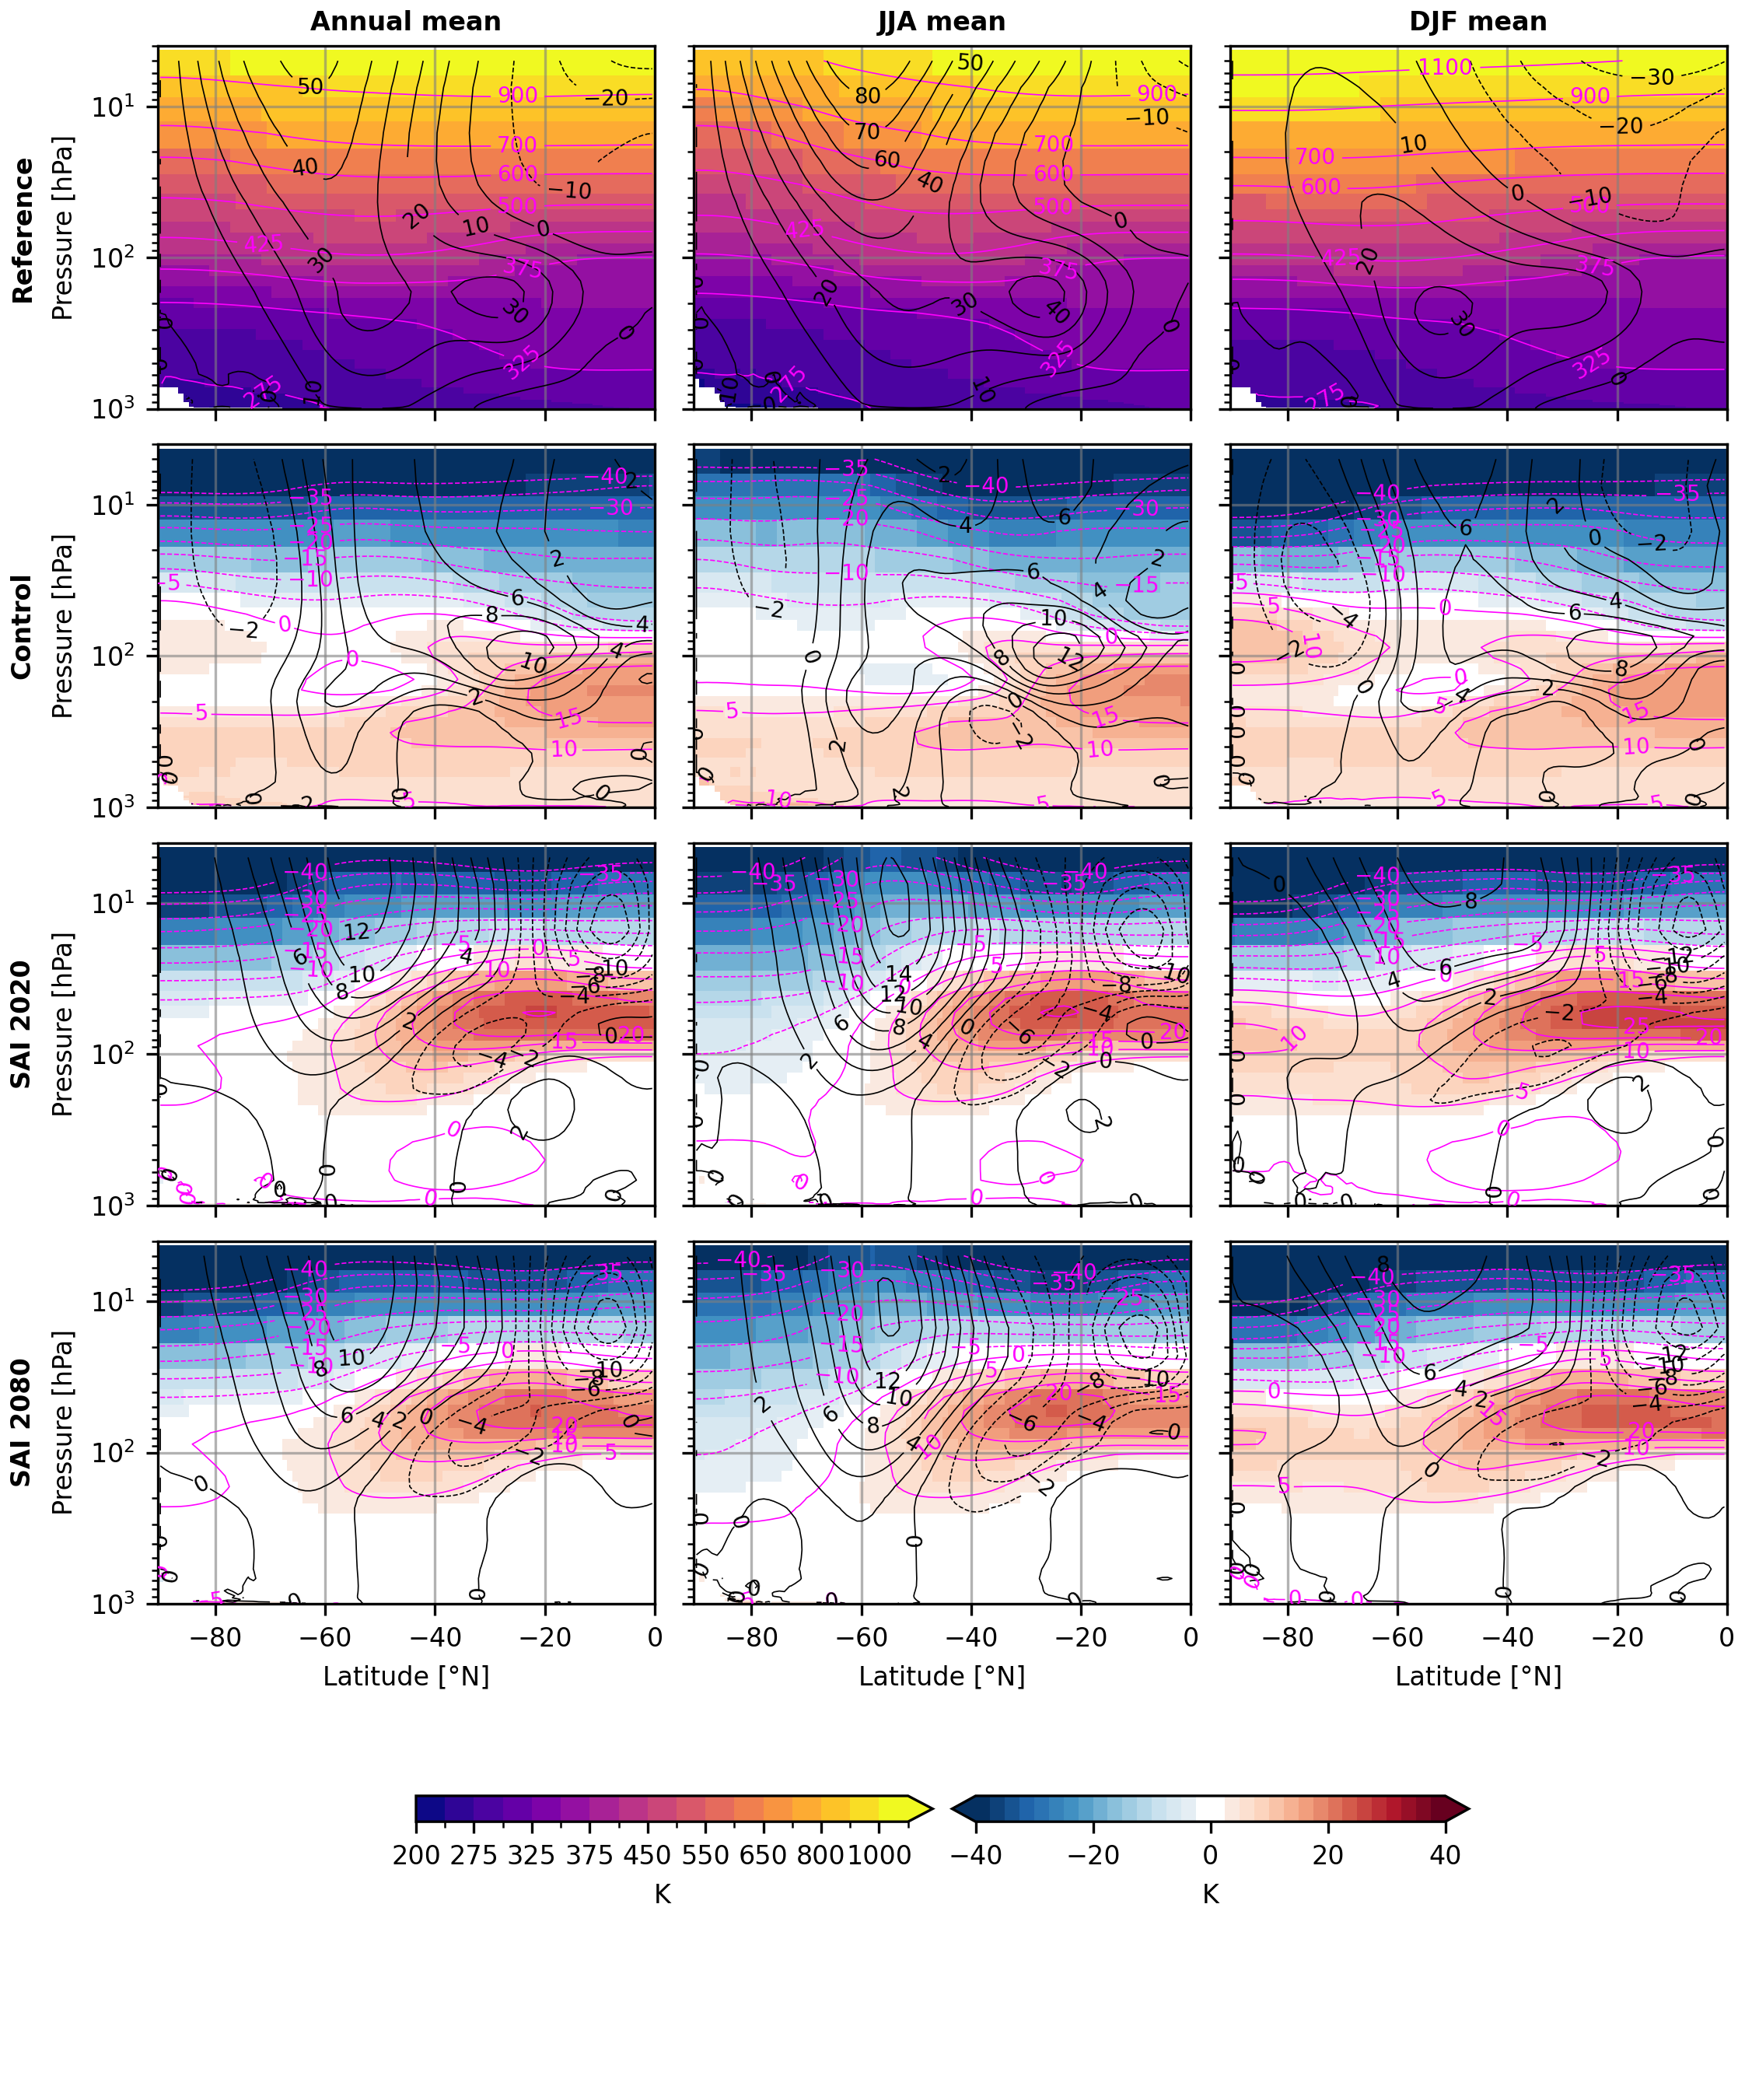
\includegraphics[width=\linewidth]{images/th_U_zmdiff_full.png}
	\caption{Annual and seasonal mean zonal-mean potential temperature (shading and magenta contours) and zonal-mean zonal wind (black contours, m/s) for Reference (first row) and Control, SAI 2020 and SAI 2080 anomaly compared to Reference (second to fourth row).}
	\label{fig:th_U_zmdiff_full}
\end{figure}

\subsection{Results Part II: Lower Stratosphere}\label{lowerstrat}

\subsubsection{Subtropical Jet}
In Figure \ref{fig:th_U_zmdiff_full} the zonal mean of the zonal component of the integrated thermal wind is shown, together with the observed zonal-mean zonal wind in black countours. The observed wind and integrated thermal wind show a strikingly similar pattern, with the observed wind consistently lower than the integrated thermal wind due to friction effects, increasingly so further up in the atmosphere. 

The change in magnitude of the lower stratosphere wind strongly correlates with the change in magnitude of the integrated thermal wind. The STJ shifts upward and equatorwad in Control, also showing a significant increase of up to 12 m/s in the upper regions. This pattern is consistent with the change in potential temperature in Figure \ref{fig:th_U_zmdiff_full}. See Figure \ref{fig:th_U_zm_JJA} in Appendix \ref{app_th_U_JJA}, the meridional gradient of the 350K isotherm is much steeper in Control compared to Reference.

In contrast, in both SAI 2020 and SAI 2080 the STJ decreases in strength, mainly in the upper regions around 100 hPa. This possibly also indicates an equatorward shift, but slightly downward instead of upward. 

On the subtropical jet intensity map in Figure \ref{fig:STJ_map_JJA} the same trends as above are observed. In Control the jet intensifies and shifts equatorward. The largest increase is observed in the easter Pacific Ocean, where in Reference the jet is relatively weak, in Control the jet is strongest in this area.

In SAI 2020 and SAI 2080 the jet is much weaker, but the spatial distribution remains largely unchanged. The jet weakens slightly more in SAI 2080 than in SAI 2020. 

jet zonality violated in 60-0 W and 0-60 E \parencite{zolotov2018variability}

% \begin{figure}[H]
% 	\centering
% 	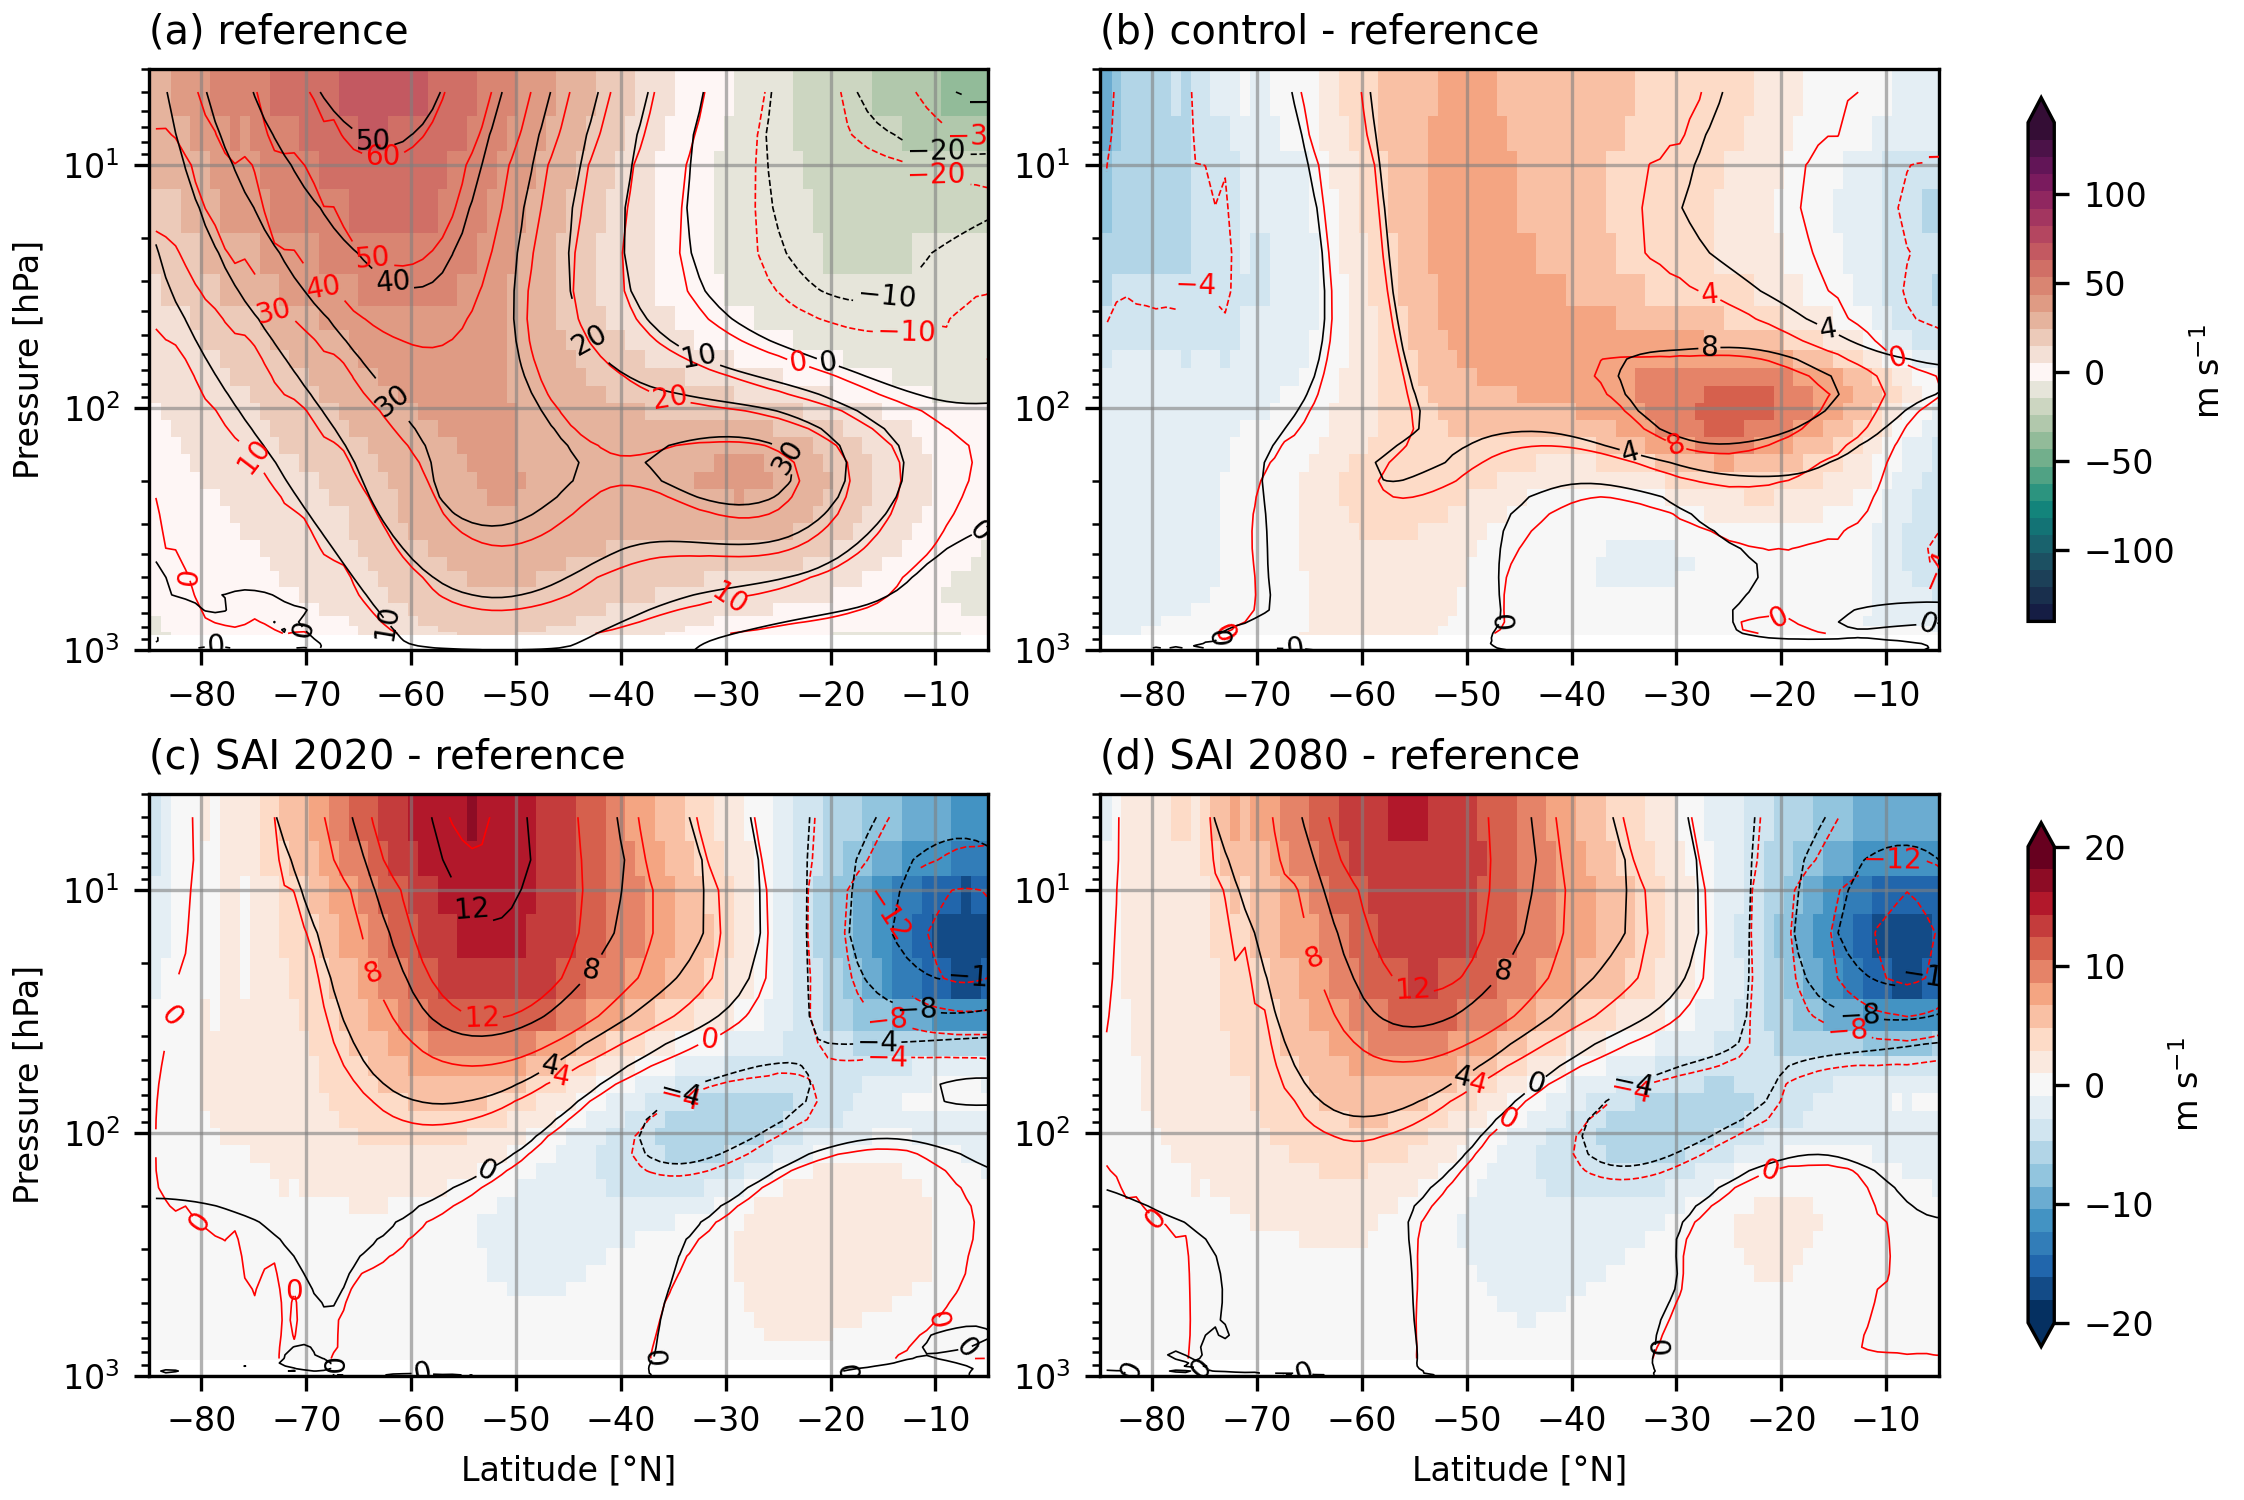
\includegraphics[width=0.95\linewidth]{images/UT_U_zmdiff_ann.png}
% 	\caption{Annual mean zonal-mean zonal thermal wind (shading and black contours) and zonal-mean zonal wind (red contours) for (a): Reference; (b-d): Control, SAI 2020 and SAI 2080 anomaly compared to Reference.}
% 	\label{fig:th_U_zmdiff_ann}
% \end{figure}

\begin{figure}[H]
	\centering
	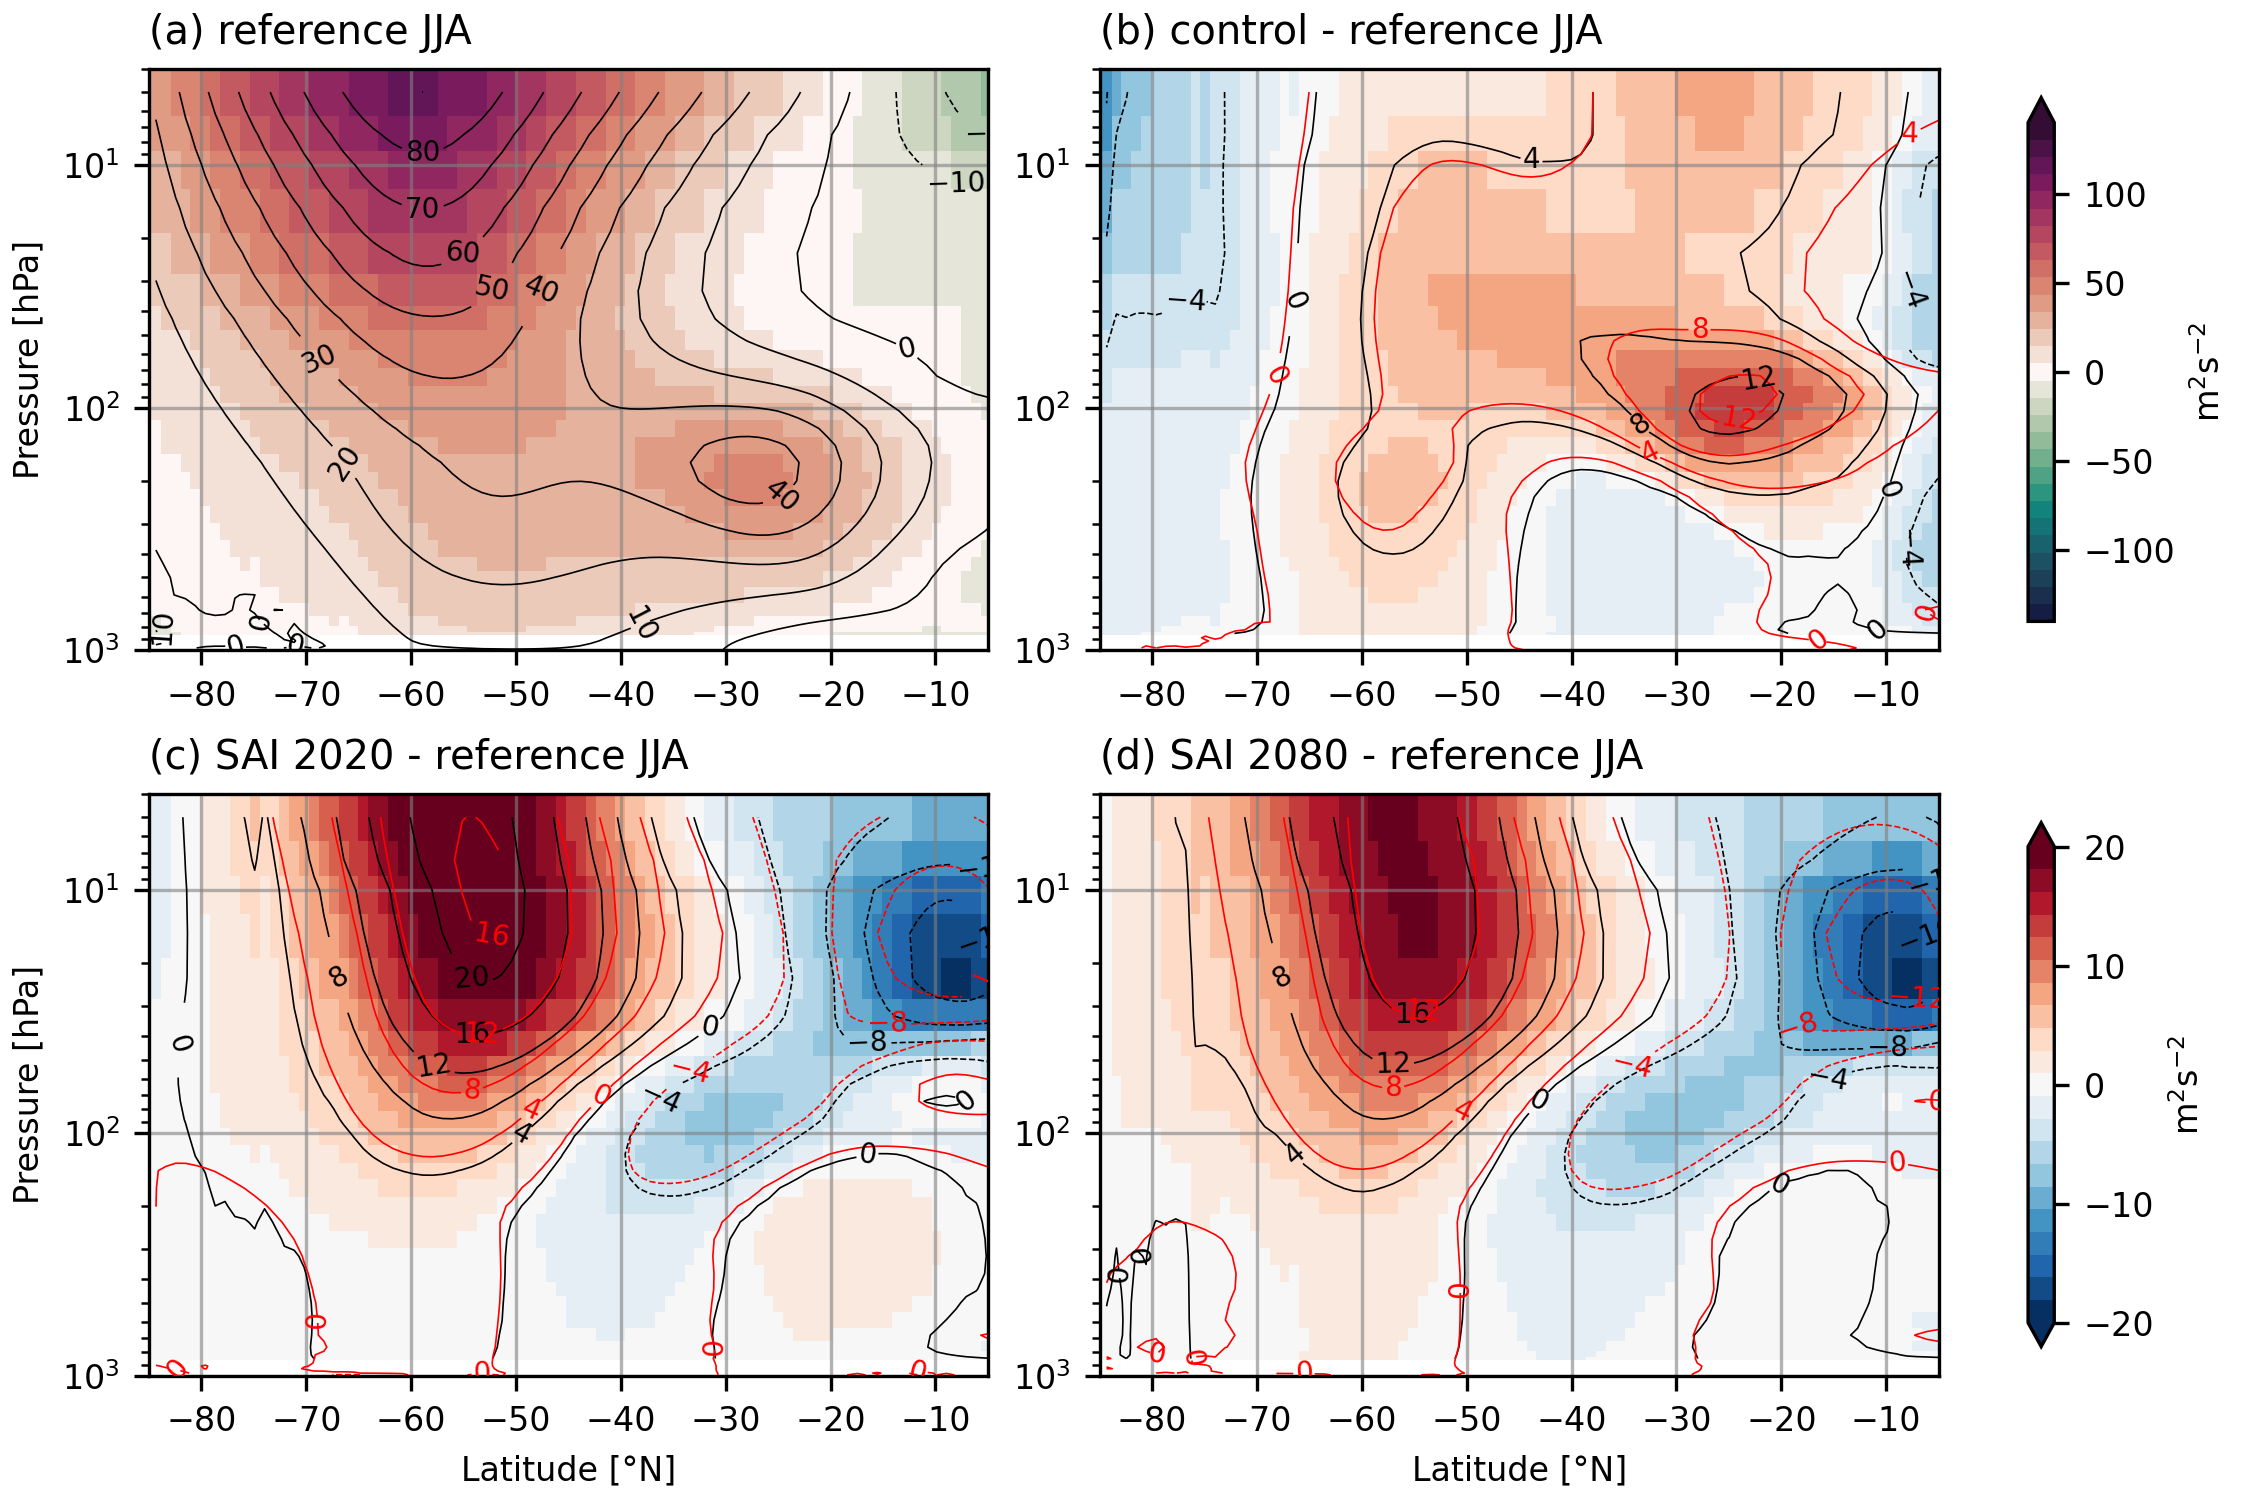
\includegraphics[width=0.95\linewidth]{images/UT_U_zmdiff_JJA.png}
	\caption{JJA mean zonal-mean zonal thermal wind (shading and red contours) and zonal-mean zonal wind (black contours, m/s) for (a): Reference; (b-d): Control, SAI 2020 and SAI 2080 anomaly compared to Reference.}
	\label{fig:UT_U_zmdiff_JJA}
\end{figure}

% \begin{figure}[H]
% 	\centering
% 	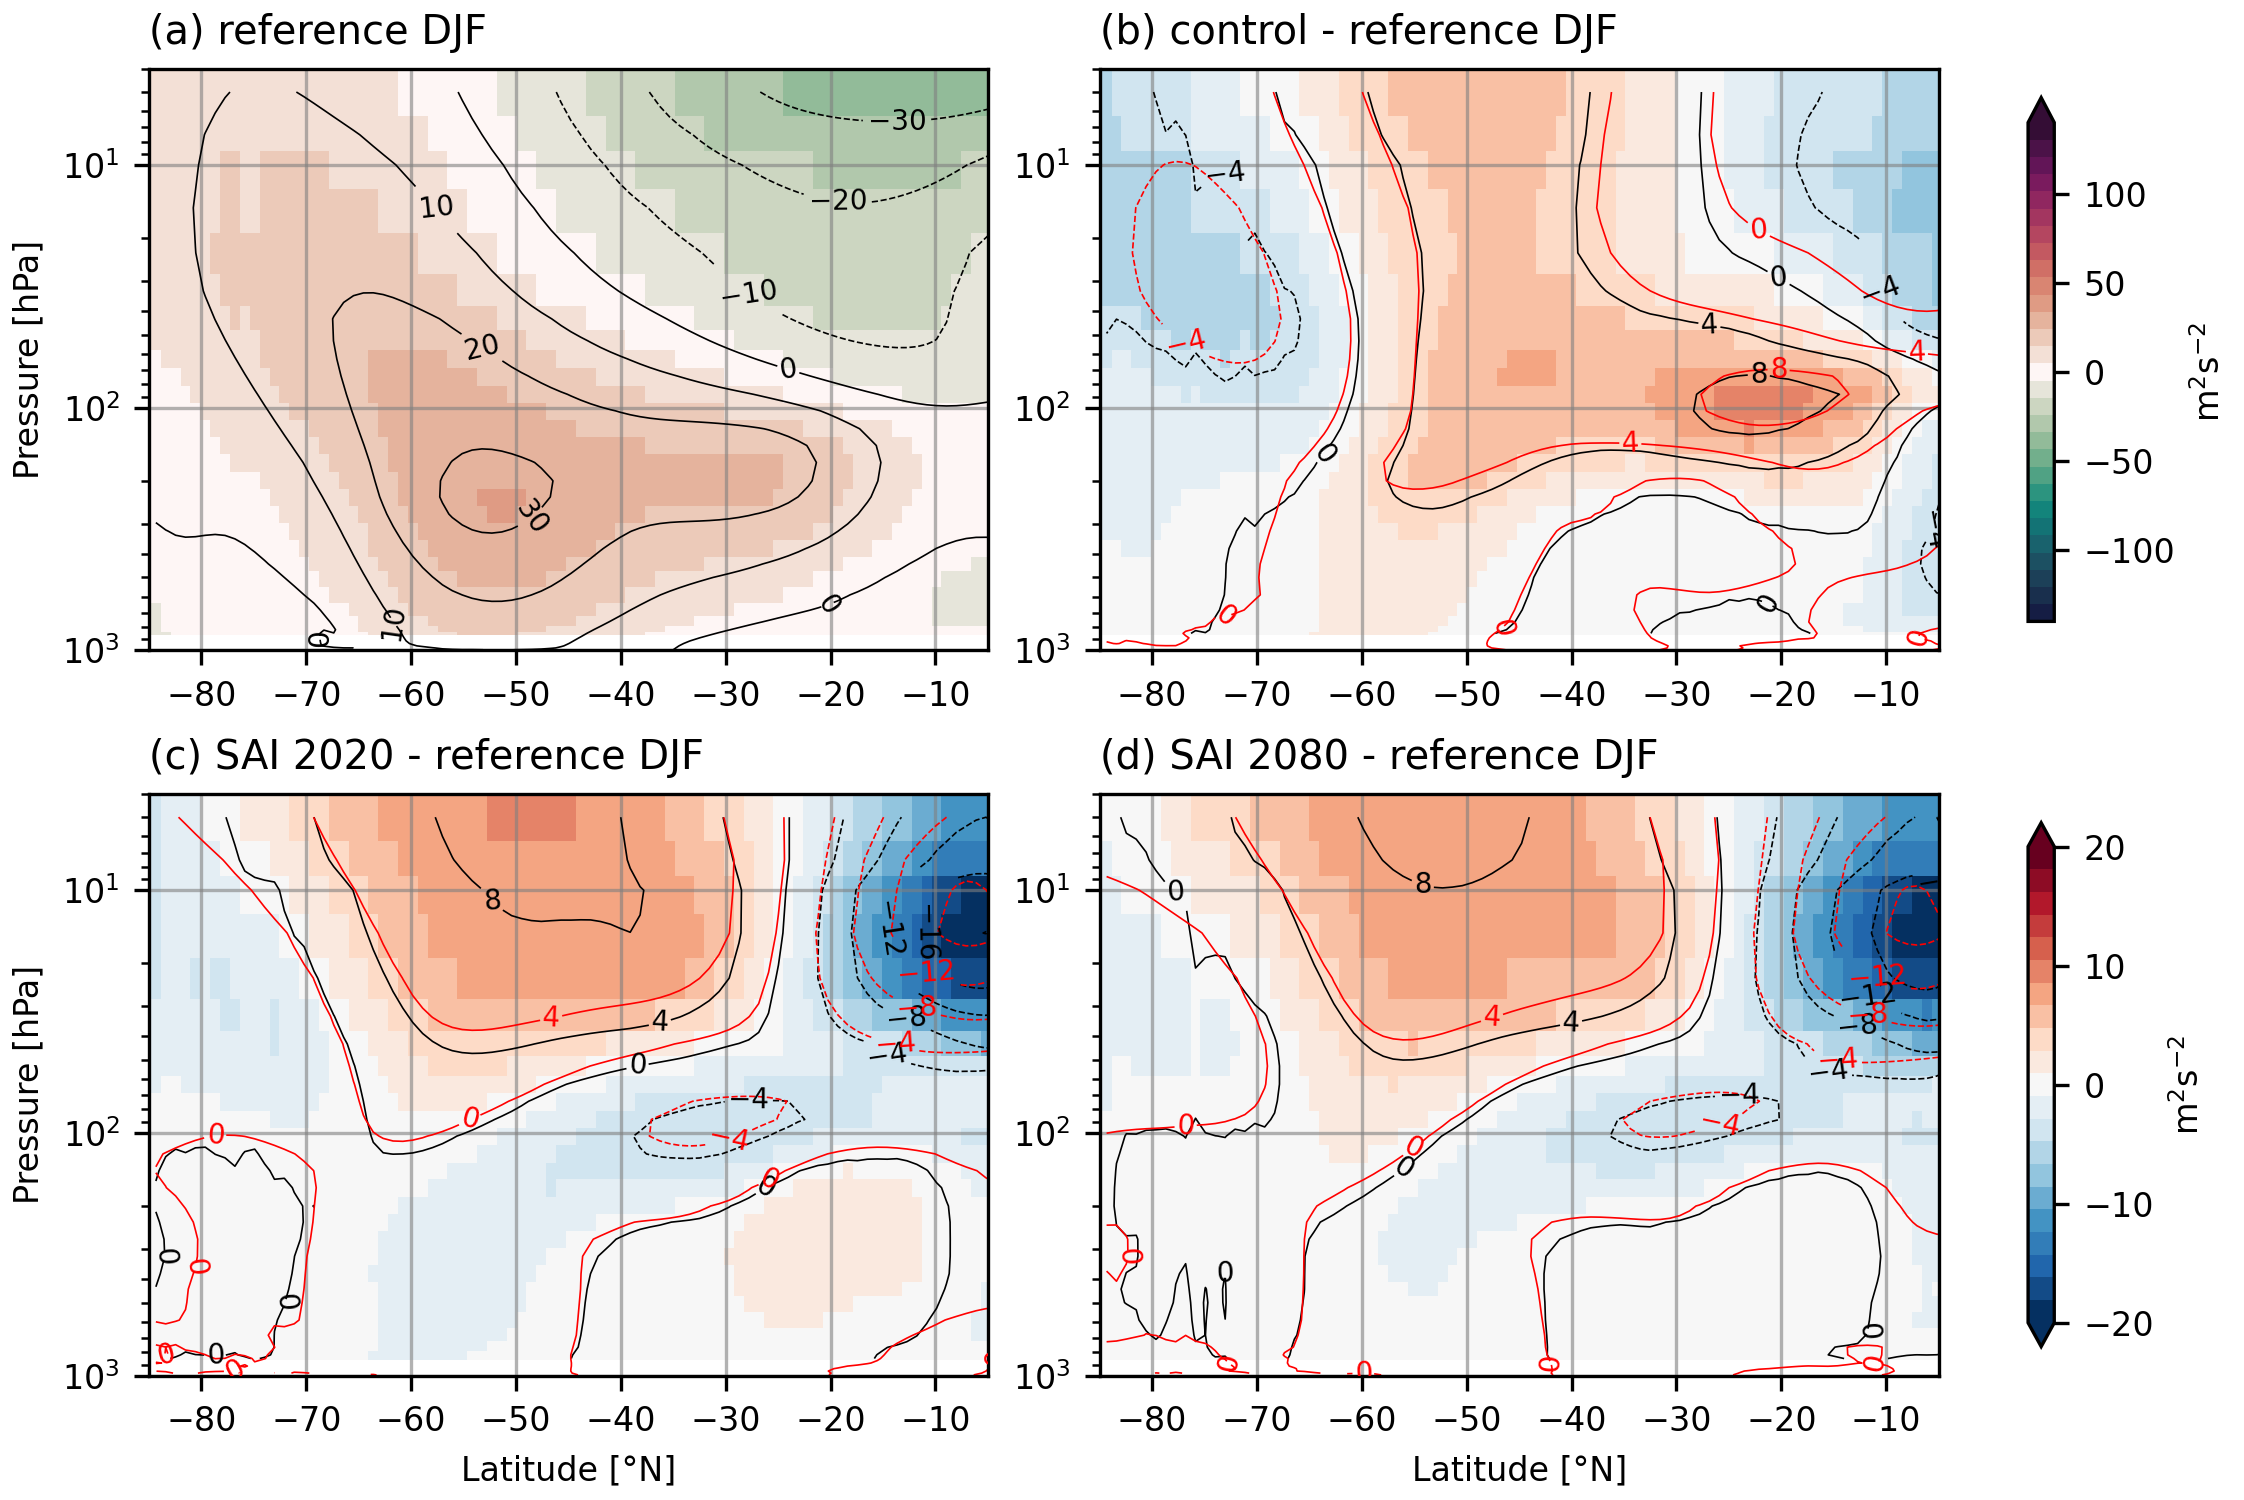
\includegraphics[width=0.95\linewidth]{images/UT_U_zmdiff_DJF.png}
% 	\caption{DJF mean zonal-mean zonal thermal wind (shading and black contours) and zonal-mean zonal wind (red contours) for (a): Reference; (b-d): Control, SAI 2020 and SAI 2080 anomaly compared to Reference.}
% 	\label{fig:th_U_zmdiff_DJF}
% \end{figure}

\begin{figure}[H]
	\centering
	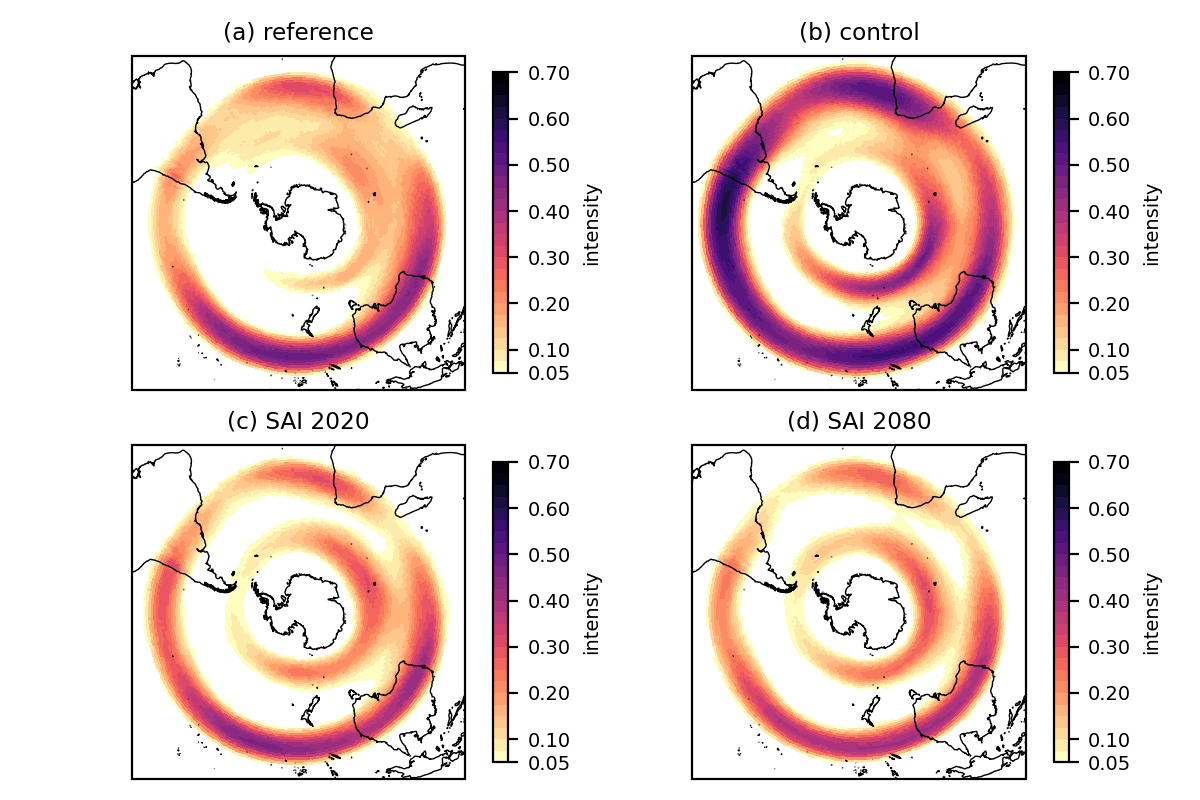
\includegraphics[width=0.95\linewidth]{images/STJ_map_JJA.png}
	\caption{JJA subtropical jet intensity map of zonal wind, values counted when the threshold of 40 m/s was passed between 400 and 100 hPa, for (a) Reference, (b) Control, (c) SAI 2020 and (d) SAI 2080.}
	\label{fig:STJ_map_JJA}
\end{figure}

\begin{figure}[H]
	\centering
	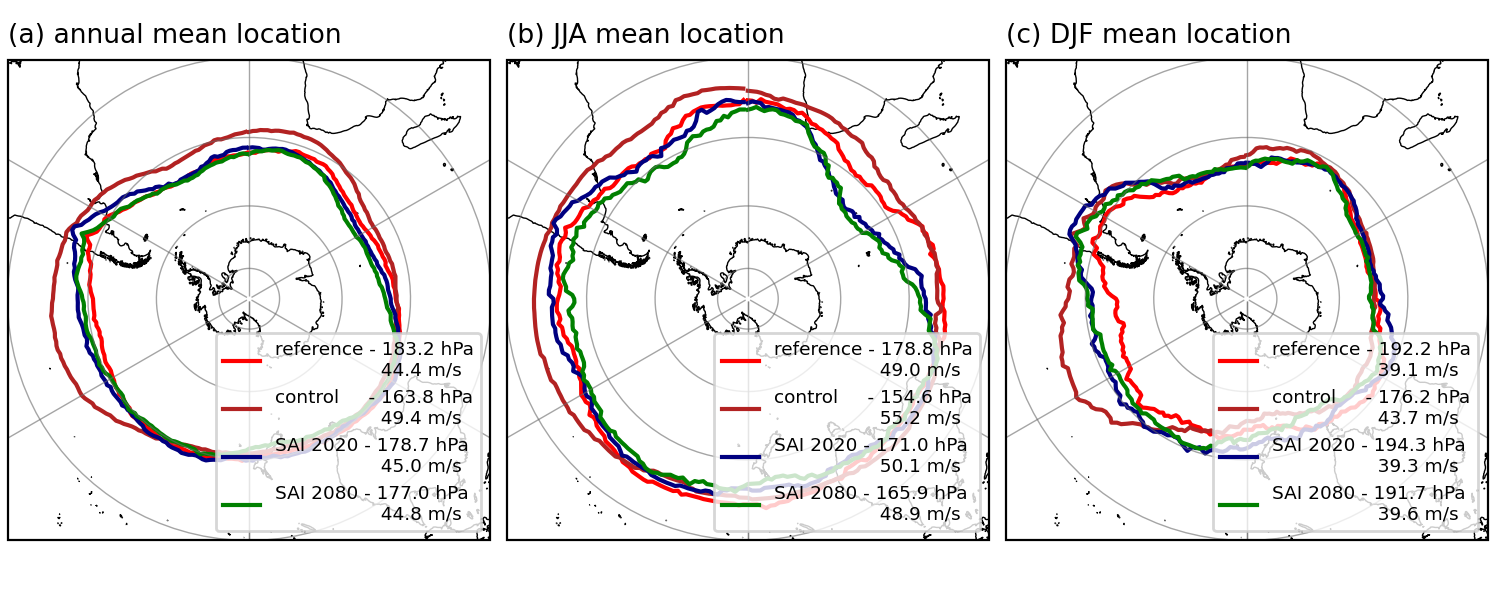
\includegraphics[width=0.95\linewidth]{images/STJ_maxloc.png}
	\caption{Mean location of the maximum of the eddy-driven jet, with corresponding longitudinal mean height and maximum eddy kinetic energy for (a) annual mean, (b) JJA mean, (c) DJF mean.}
	\label{fig:STJ_maxloc}
\end{figure}


\subsubsection{Eddy-driven Jet}\label{EDJ_sec}
More poleward, around 50°S, another jet structure appears, mostly visible in Figure \ref{fig:STJ_map_JJA}. The zonal wind in this area increases, most notably in Control, which is also visible in Figure \ref{fig:th_U_zmdiff_full}. Beacuse this jet is driven by eddy activity, the zonal-mean eddy kinetic energy (EKE) and EKE anomalies are shown in Figure \ref{fig:EKE_U_zmdiff_JJA}.

Around 50°S and 300 hPa, there is a peak in EKE, i.e. high eddy activity. In Control the EKE decreases on the lower equatorward side of the jet and increases on the upper poleward side, indicating that the jet shifts poleward and upward. In SAI 2020 and SAI 2080 the EKE shows small changes relative to Control, with the most notable change the decrease around 45°S, right in between the EDJ and the STJ. 

The eddy-driven jet intensity map in Figure \ref{fig:EDJ_map_JJA} is also shown to increase in intensity in Control and slightly decrease in both SAI 2020 and SAI 2080. The spatial pattern remains largely unchanged in all scenarios. 

\begin{figure}[H]
	\centering
	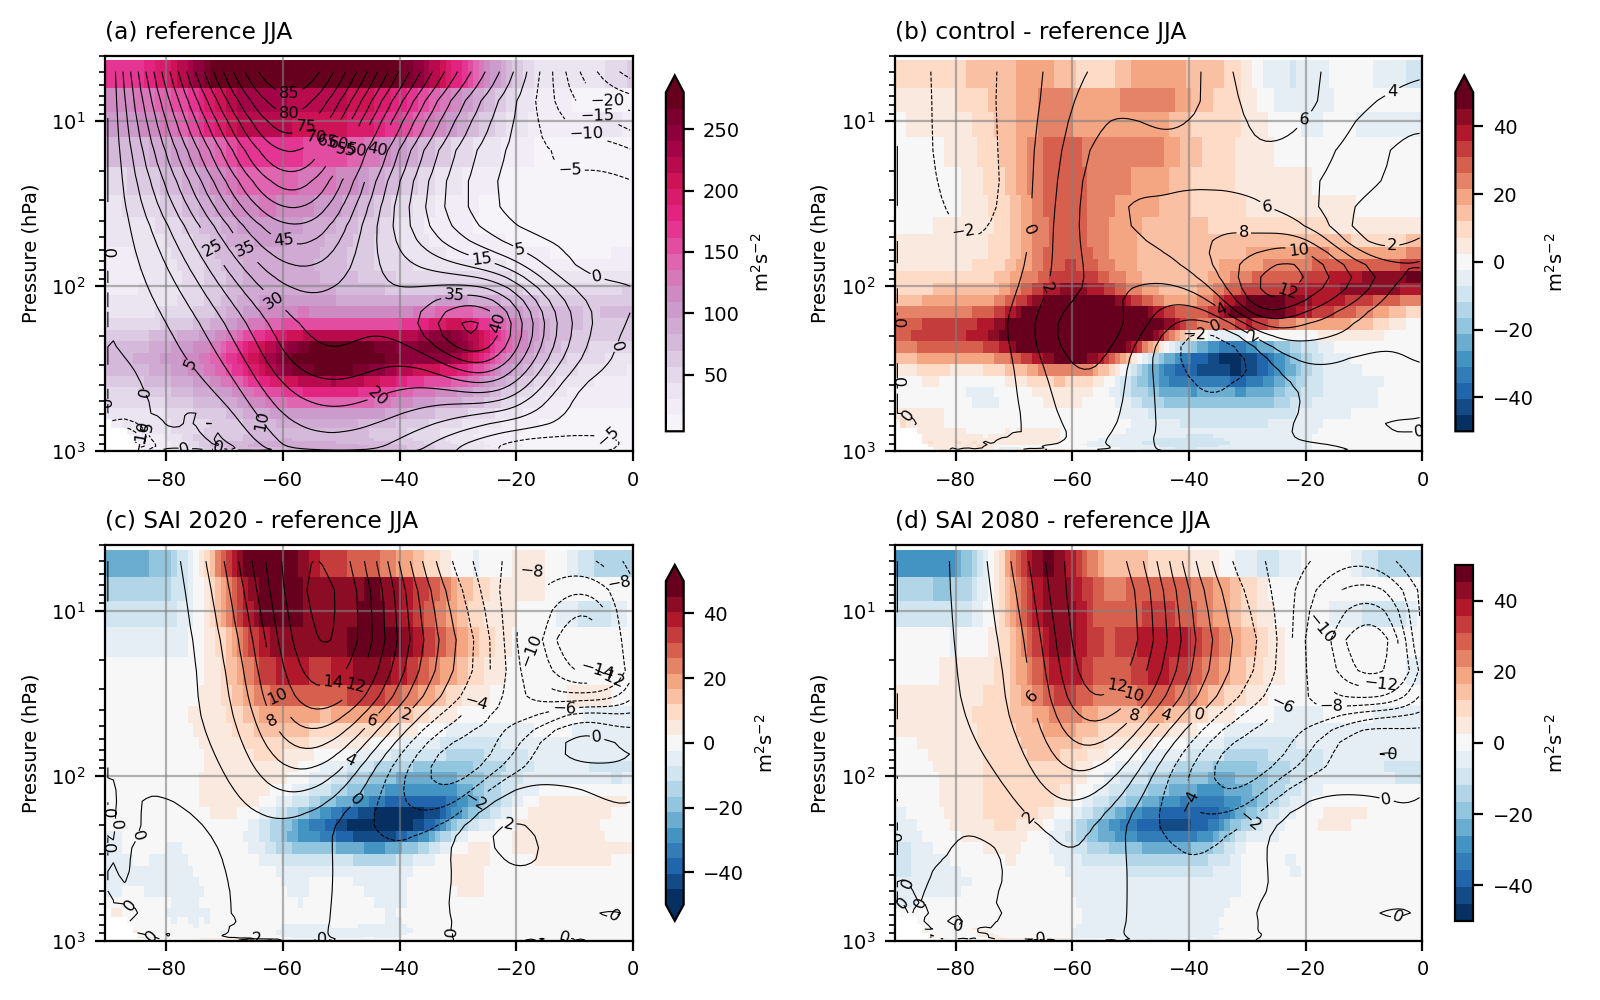
\includegraphics[width=0.95\linewidth]{images/EKE_U_zmdiff_JJA.png}
	\caption{JJA mean zonal-mean eddy kinetic energy (shading) and zonal-mean zonal wind (contours, m/s) for (a): Reference; (b-d): Control, SAI 2020 and SAI 2080 anomaly compared to Reference.}
	\label{fig:EKE_U_zmdiff_JJA}
\end{figure}

\begin{figure}[H]
	\centering
	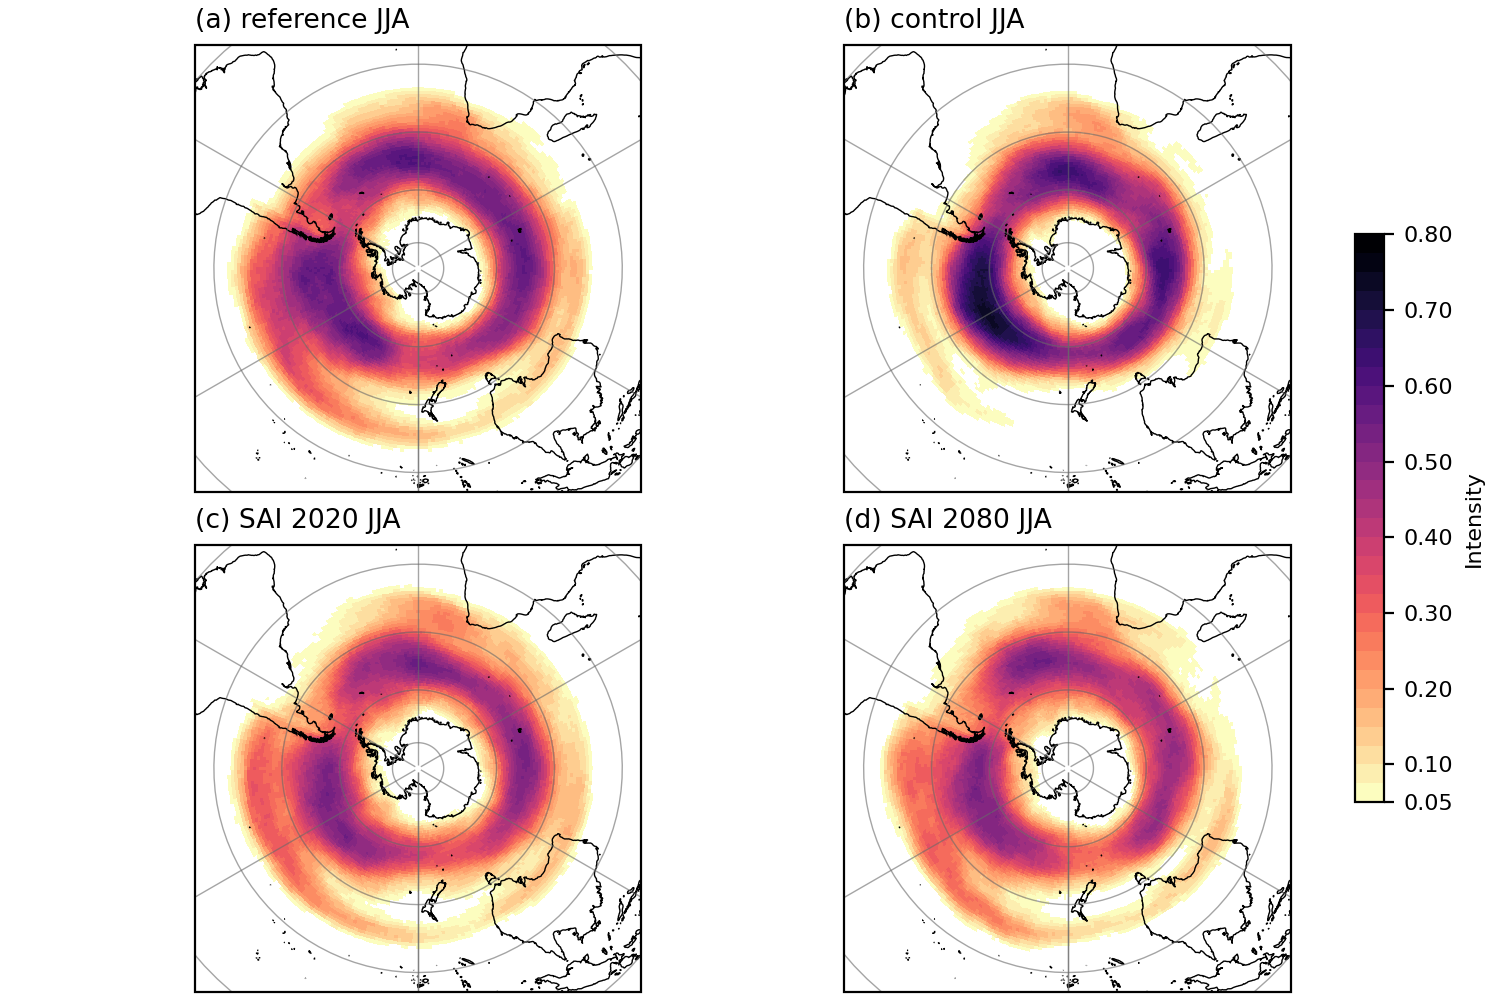
\includegraphics[width=0.95\linewidth]{images/EDJ_map_JJA.png}
	\caption{JJA eddy-driven jet intensity map of EKE, values counted when the threshold of 105 J/m$^3$ was passed between 600 and 150 hPa, for (a) Reference, (b) Control, (c) SAI 2020 and (d) SAI 2080.}
	\label{fig:EDJ_map_JJA}
\end{figure}

\begin{figure}[H]
	\centering
	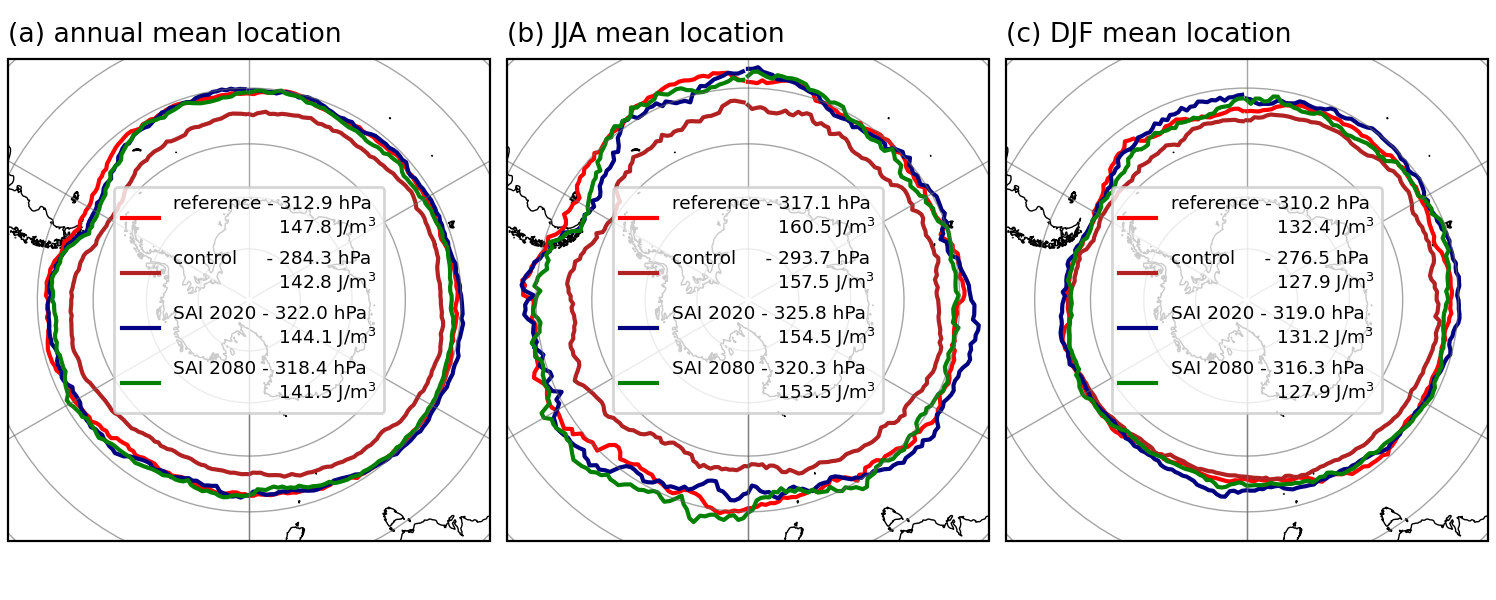
\includegraphics[width=0.95\linewidth]{images/EDJ_maxloc.png}
	\caption{Mean location of the maximum of the eddy-driven jet, with corresponding mean height and mean maximum eddy kinetic energy, (a) annual mean, (b) JJA mean, (c) DJF mean.}
	\label{fig:EDJ_maxloc}
\end{figure}

There is a clear correlation between the EKE anomalies and zonal-mean zonal wind anomalies, thus we look at the kinetic energy to disentangle the change in zonal wind from the change in EKE. In Figure \ref{fig:KE_U_zmdiff_JJA} the zonal-mean kinetic energy and zonal-mean zonal wind are shown. 

For Control the increase in KE energy follows the zonal wind patterns in sign, but not in magnitude. The KE increases with the increasing zonal wind accordingly in the upper regions of the STJ, but the KE increases and decreases more in the EDJ area than would be expedted from the increase in zonal wind. 

For SAI 2020 and SAI 2080 the KE anomaly does follow the zonal wind anomaly proportionally and comparison with Figure \ref{fig:EKE_U_zmdiff_JJA} shows that the decrease in EKE is correlated with the decrease in zonal wind. This correlation is also clear when comparing the jet intensity maps in Figures \ref{fig:STJ_map_JJA} and \ref{fig:EDJ_map_JJA}.

\begin{figure}[H]
	\centering
	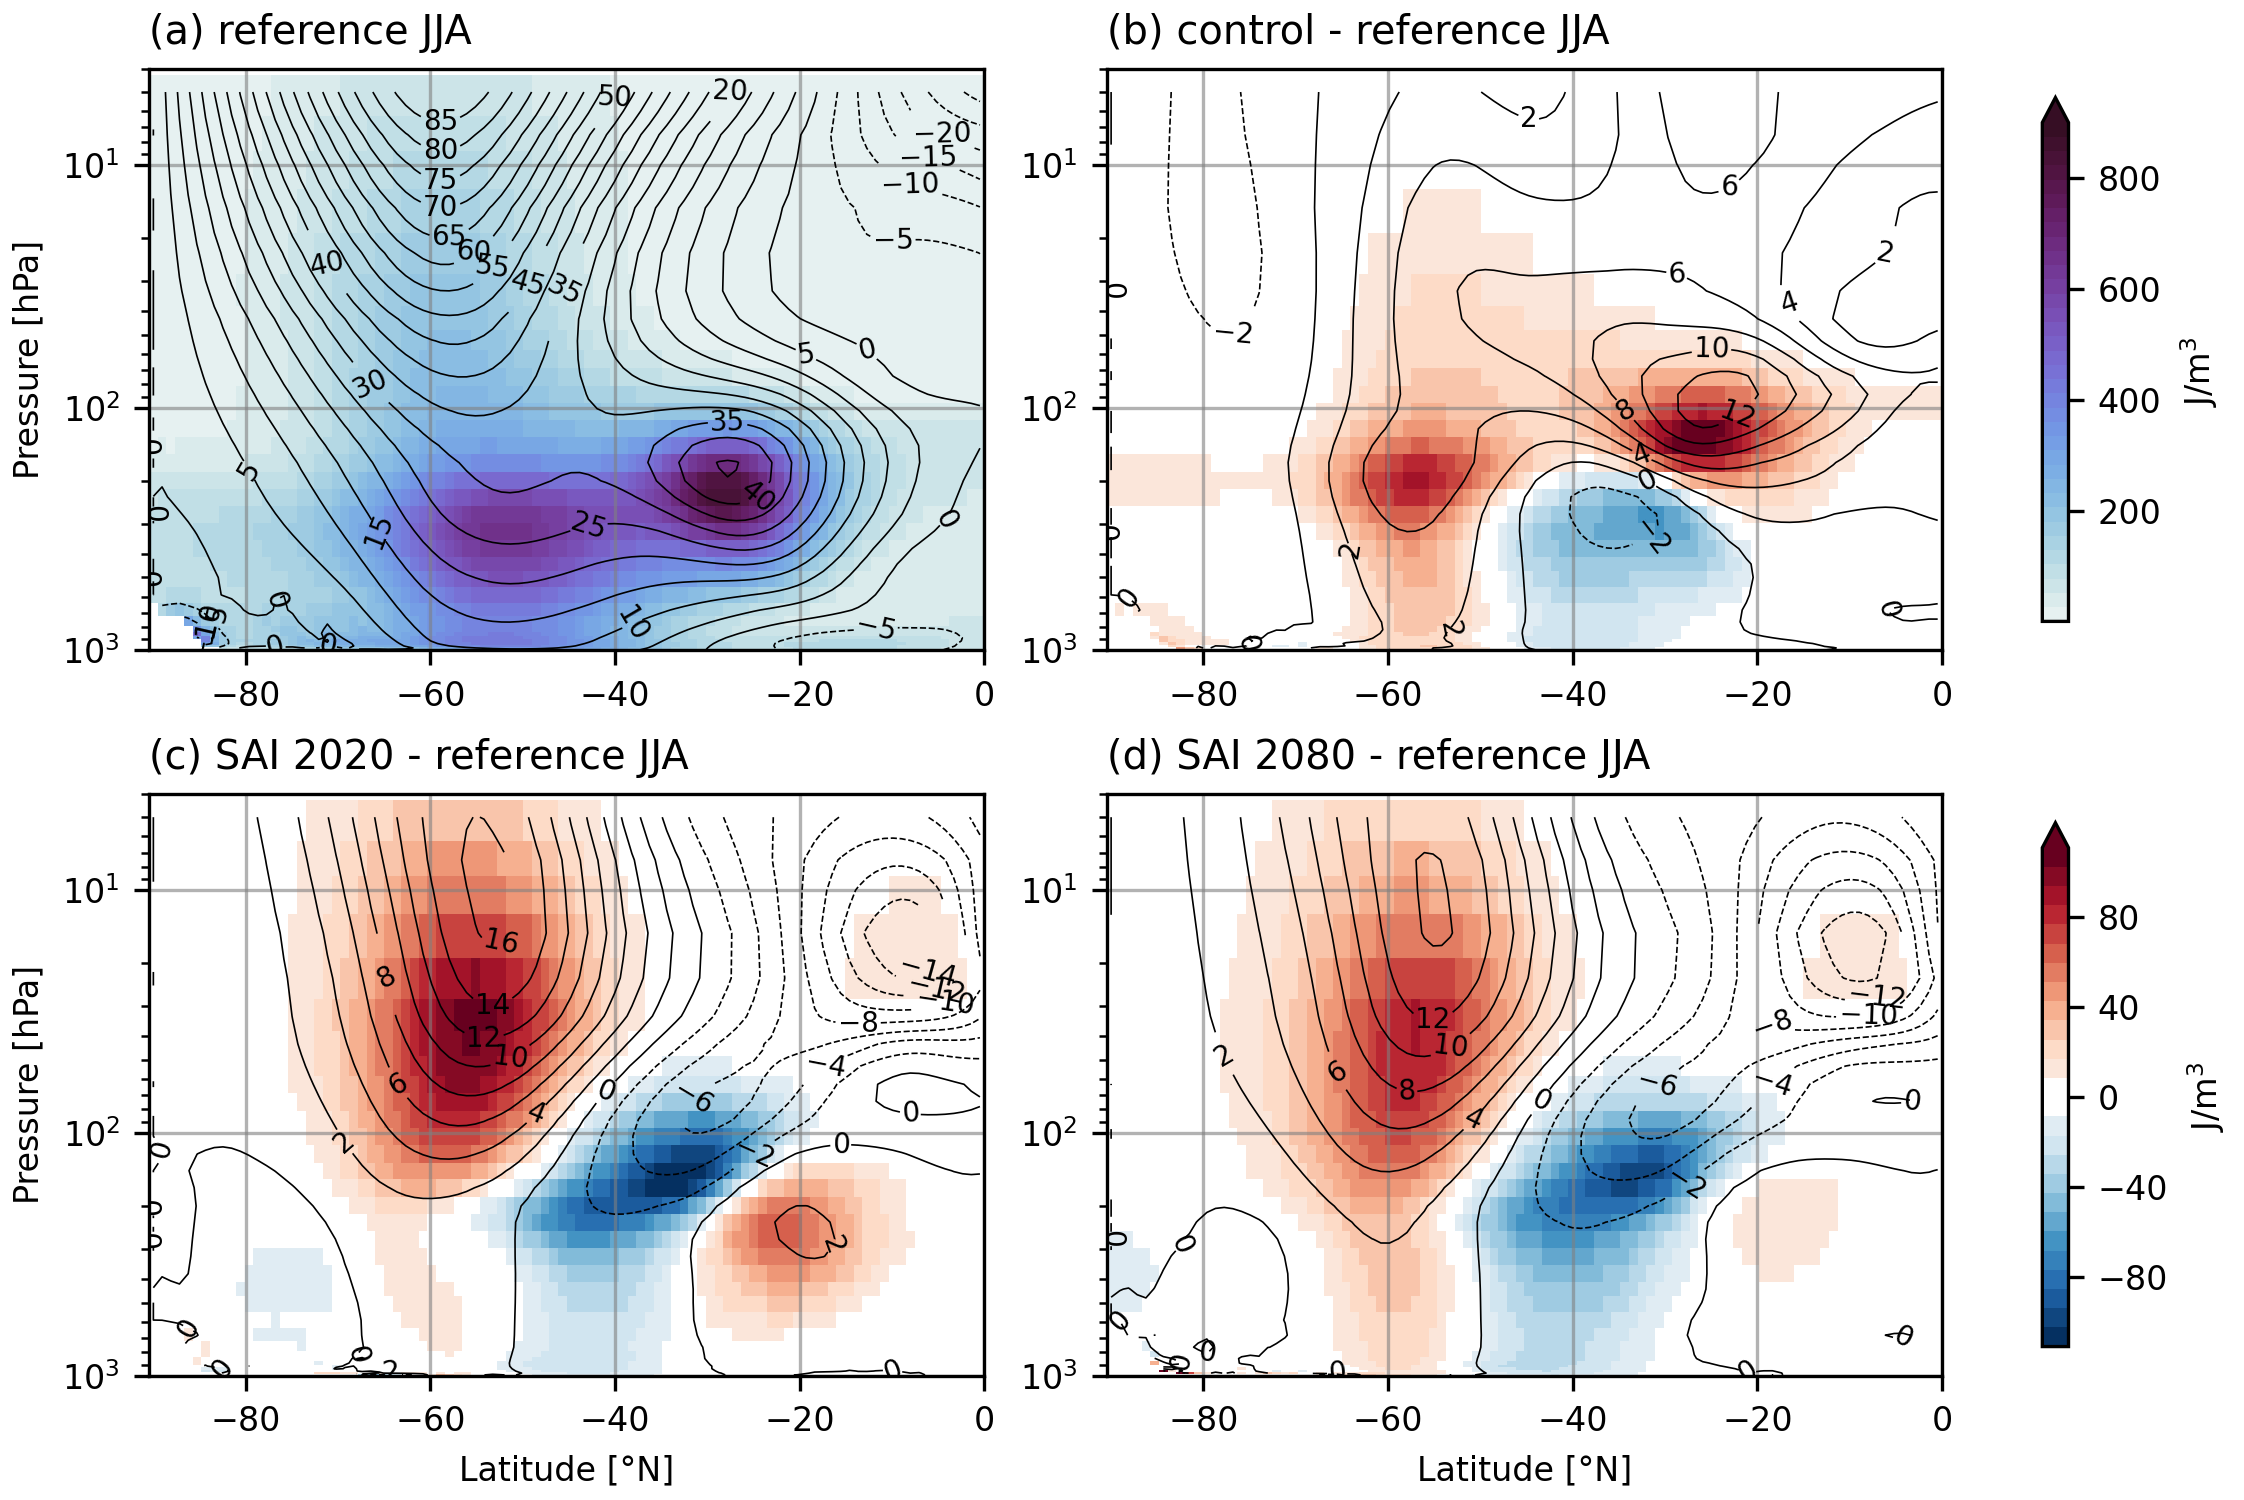
\includegraphics[width=0.95\linewidth]{images/KE_U_zmdiff_JJA.png}
	\caption{JJA mean zonal-mean kinetic energy (shading) and zonal-mean zonal wind (contours, m/s) for (a): Reference; (b-d): Control, SAI 2020 and SAI 2080 anomaly compared to Reference.}
	\label{fig:KE_U_zmdiff_JJA}
\end{figure}

